When it comes to preventing in-process memory abuse, developers are virtually helpless due to a lack of support from underlying operating systems (OS): the memory isolation mechanisms provided by modern OS operate merely at the process level and cannot be used to establish security boundaries inside a process. As a result, protecting sensitive memory content against malicious code inside the same process remains an open issue, which has been increasingly exploited by attackers.

\begin{figure}[h]
\begin{center}
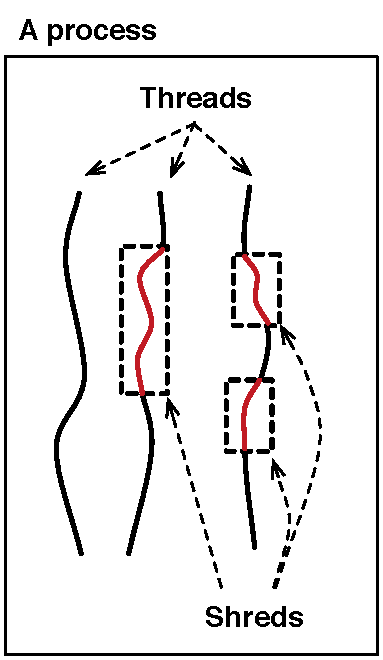
\includegraphics[scale=0.55]{shreds/figures/shreds}
\caption{Shreds, threads, and a process}
\label{fig:shred}
\end{center}
\end{figure}
\subsection{Overview}
\label{shreds:sec:overview}

%
%To address this open issue, some recent work proposed the thread-level memory isolation~\cite{wedge}, which allows developers to limit the sharing of a thread's memory space with other threads in the same process. However, this line of works faces three major limitations. First, thread-level memory isolation is still too coarse to stop in-process abuse because exploitable or malicious code often run in the same thread as the legitimate code that needs to access sensitive memory content. Second, adopting these solutions requires significant efforts from developers. Separating application components into different threads (i.e., scheduling units) demands major design changes, as opposed to regional code patches, to deal with the added concurrency. Third, threads with private memory tend to incur much higher overhead than normal threads due to the additional page table switches, TLB flushes, or nested page table management upon context switches. We aim to tackle these challenges by proposing a practical and effective system to realize in-process private memory.

In this section, we present a new execution unit for userspace code, namely shred, which represents an arbitrarily sized segment of a thread (hence the name) and is granted exclusive access to a protected memory pool, namely shred-private pool (or s-pool). Figure~\ref{fig:shred} depicts shreds in relation to the conventional execution units. Upon its creation, a shred is associated an s-pool, which can be shared among multiple shreds. Shreds address developers' currently unmet needs for fine-grained, convenient, and efficient protection of sensitive memory content against in-process adversaries. To prevent sensitive content in memory from in-process abuse, a developer includes into a shred the code that needs access to the sensitive content and stores the content in the shred's s-pool. For instance, an encryption function can run in a shred with the secret keys stored in the s-pool; a routine allowed to call a private API can run in a shred whose s-pool contains the API code.


We design \shreds under a realistically adversarial threat model. We assume attackers may have successfully compromised a victim program, via either remote exploitation or malicious local libraries. Attackers' goal is to access the sensitive content, including both data and code, in the victim program's virtual memory space. Further, we expect unknown vulnerabilities to exist inside shreds (e.g., control flow hijacks and data leaks are possible). On the other hand, we assume a clean OS, which serves as the TCB for shreds. The assumption is reasonable because the attacks that shreds aim to prevent, in-process abuse, would become unnecessary had attackers already subverted the OS. In fact, we advocate that, future OS should support shreds, or more generally, enable private memory for execution units of smaller granularities than the scheduling units.

We realize the concept of shreds by designing and building: (\rom{1}) a set of easy-to-use APIs for developers to use shreds and s-pools; (\rom{2}) a compilation toolchain, called S-compiler, automatically verifying, instrumenting, and building programs using shreds; (\rom{3}) a loadable kernel extension, called S-driver, enabling the support and protection of shreds on commodity OS. Figure~\ref{fig:overview} shows an overview of the entire system and the workflow. A developer creates a shred and associates it with a selected s-pool by calling the shred enter API and supplying the s-pool descriptor as the argument. Code inside a shred may access content in the associated s-pool as if it were a normal region in the virtual memory space. But the s-pool is inaccessible outside of the associated shred(s). S-pools are managed and protected by S-driver in a way oblivious to developers or applications. With the help of use-define chain analysis on labeled sensitive variables, shreds can also be created automatically at compile time.

As shown in Figure~\ref{fig:overview}, while compiling programs that use shreds, S-compiler automatically verifies the safe usage of shreds and instruments in-shred code with inline checks. The verification and instrumentation regulate sensitive data propagation and control flows inside shreds so that unknown vulnerabilities inside shreds cannot lead to secret leaks or shred hijacking. During runtime, S-driver serves as the manager for s-pools and the security monitor for executing shreds. It creates and resizes s-pools on demand. It enables a per-CPU locking mechanism on s-pools and ensures that only authorized shreds may access s-pools despite concurrent threads.
S-driver leverages an under-exploited CPU feature, namely ARM memory domains~\cite{domains}, to efficiently realize s-pools and enforce shred-based access control. Unlike the previously proposed thread-level memory isolations~\cite{wedge}, our approach neither requires separate page tables nor causes additional page table switches or full TLB flushes. Our approach also avoids the need for a hypervisor or additional levels of address translates (e.g., nested paging). Although our reference design and implementation of s-pools are based on ARM CPUs, they are compatible with future x86 architectures, which will be equipped with a feature similar to memory domain~\cite{mpk15,mpk:rfc}.

We implement S-compiler based on LLVM~\cite{lattner2004llvm} and S-driver as a kernel module for Linux. We evaluate shreds' compatibility and the ease of adoption by manually retrofitting shreds into 5 non-trivial open source software, including OpenSSL and Lighttpd. We show that developers can easily adopt shreds in their code without design-level changes or sacrifice of functionality. Our evaluation shows that shreds incurs an average end-to-end overhead of 4.67\%. We also conduct security analysis on shreds, confirming that possible attacks allowed in our thread model are prevented. Overall, our results indicate that shreds can be easily adopted in real software for fine-grained protection of sensitive memory content while incurring very low overhead.

\begin{figure*}[t]
\begin{center}
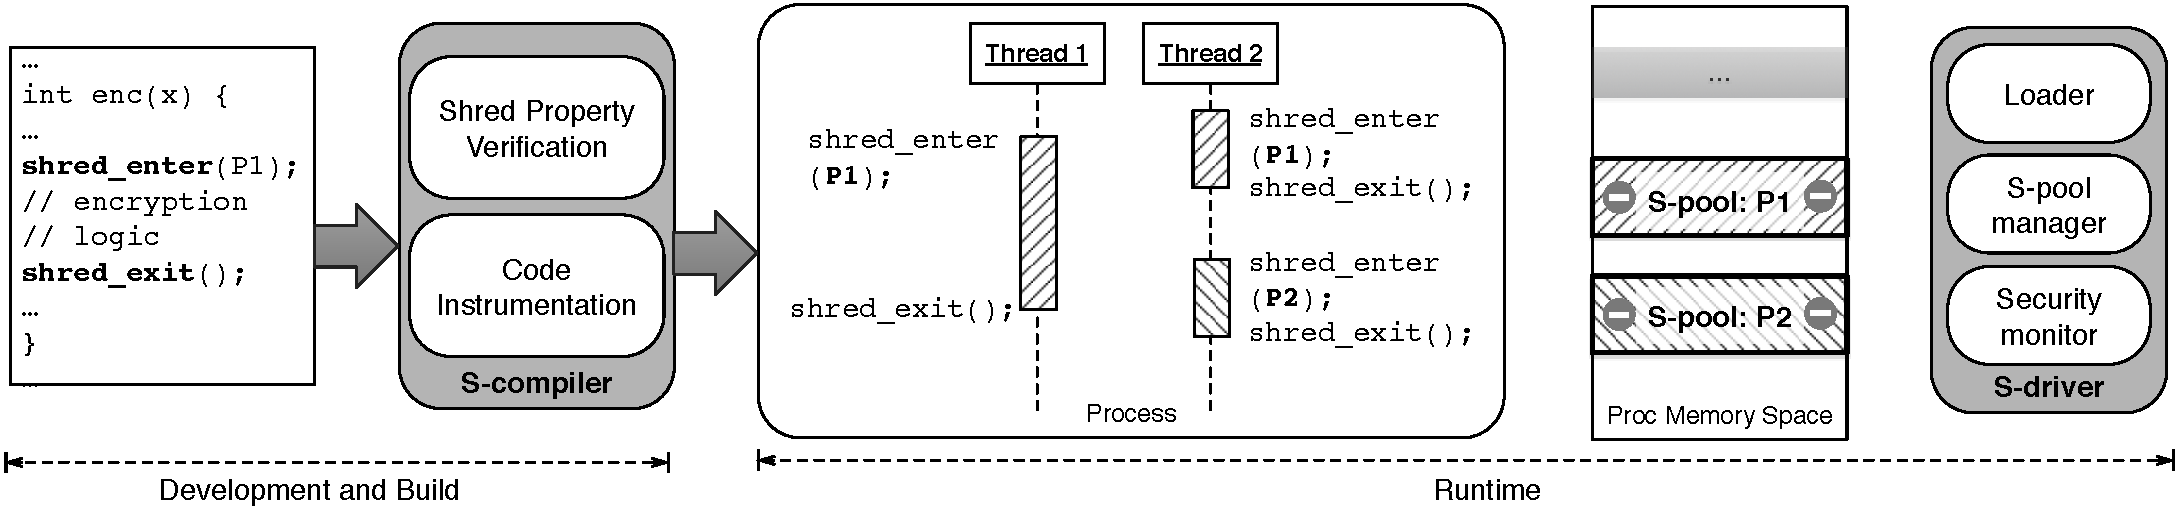
\includegraphics[scale=0.45]{shreds/figures/arch}
%\caption{System Overview}
\caption{Developers create shreds in their programs via the intuitive APIs and build the programs using S-compiler, which automatically verifies and instruments the executables (left); during runtime (right), S-driver handles shred entrances and exits on each CPU/thread while efficiently granting or revoking each CPU's access to the s-pools.}
\label{fig:overview}
\end{center}
\end{figure*}
